%----------------------------------------------------------------------------------------
%	Inställningar och dokumentkonfiguration
%----------------------------------------------------------------------------------------

\documentclass[paper=a4, fontsize=11pt]{report} % A4-sida och 11 punkters fontstorlek

\usepackage[T1]{fontenc} % 8-bitarskodning som har 256 glyfer
\usepackage[english]{babel} % Svenskt språk
\usepackage[utf8]{inputenc} % För svenska tecken
\usepackage{dtklogos} % Logos
\usepackage{wallpaper} % Bakgrundsbild
\usepackage{fancyhdr} % Specialsidhuvud och sidfot
\usepackage{enumerate} 
\usepackage{xifthen}% provides \isempty test
\usepackage{listings}% Code examples
\usepackage{xcolor}
\newcounter{tmpc}
\lstdefinestyle{BashInputStyle}{
  language=bash,
  basicstyle=\footnotesize\ttfamily,
  numbers=left,
  numberstyle=\tiny,
  numbersep=3pt,
  frame=tb,
  columns=fullflexible,
  backgroundcolor=\color{yellow!20},
  linewidth=0.9\linewidth,
  xleftmargin=0.1\linewidth
}
% Exampels
% Inline
% \lstinline[style=BashInputStyle]´# apt-get --purge remove rubygems´.
% Multiline
% \begin{lstlisting}[style=BashInputStyle]
%    # apt-get --purge remove rubygems
% \end{lstlisting}

\pagestyle{fancyplain} % Använd sidhuvud och sidfot på alla sidor
\fancyhead[L]{Seminar 4 -- 1DV020 -- 2015 -- Server Administration} % Titel till vänster i sidhuvud
\fancyhead[C]{} % Tomt i mitten
\fancyhead[R]{} % Tomt till höger
\fancyfoot[L]{} % Tomt till vänster
\fancyfoot[C]{} % Tomt i mitten
\fancyfoot[R]{\thepage} % Sidnumrering till höger i sidfoten
\renewcommand\thesection{\arabic{section}} % Section beter sig som i dokumentklassen article

\newcommand{\win}[1]{Microsoft Windows Server\ifthenelse{\isempty{#1}}{}{ #1}}
\newcommand{\gui}[0]{``Server with a GUI''}
\newcommand{\core}[0]{Windows Server Core}
%----------------------------------------------------------------------------------------
%	TITLE SECTION
%----------------------------------------------------------------------------------------
\newcommand\BackgroundPic{
    \put(-50,-50){
    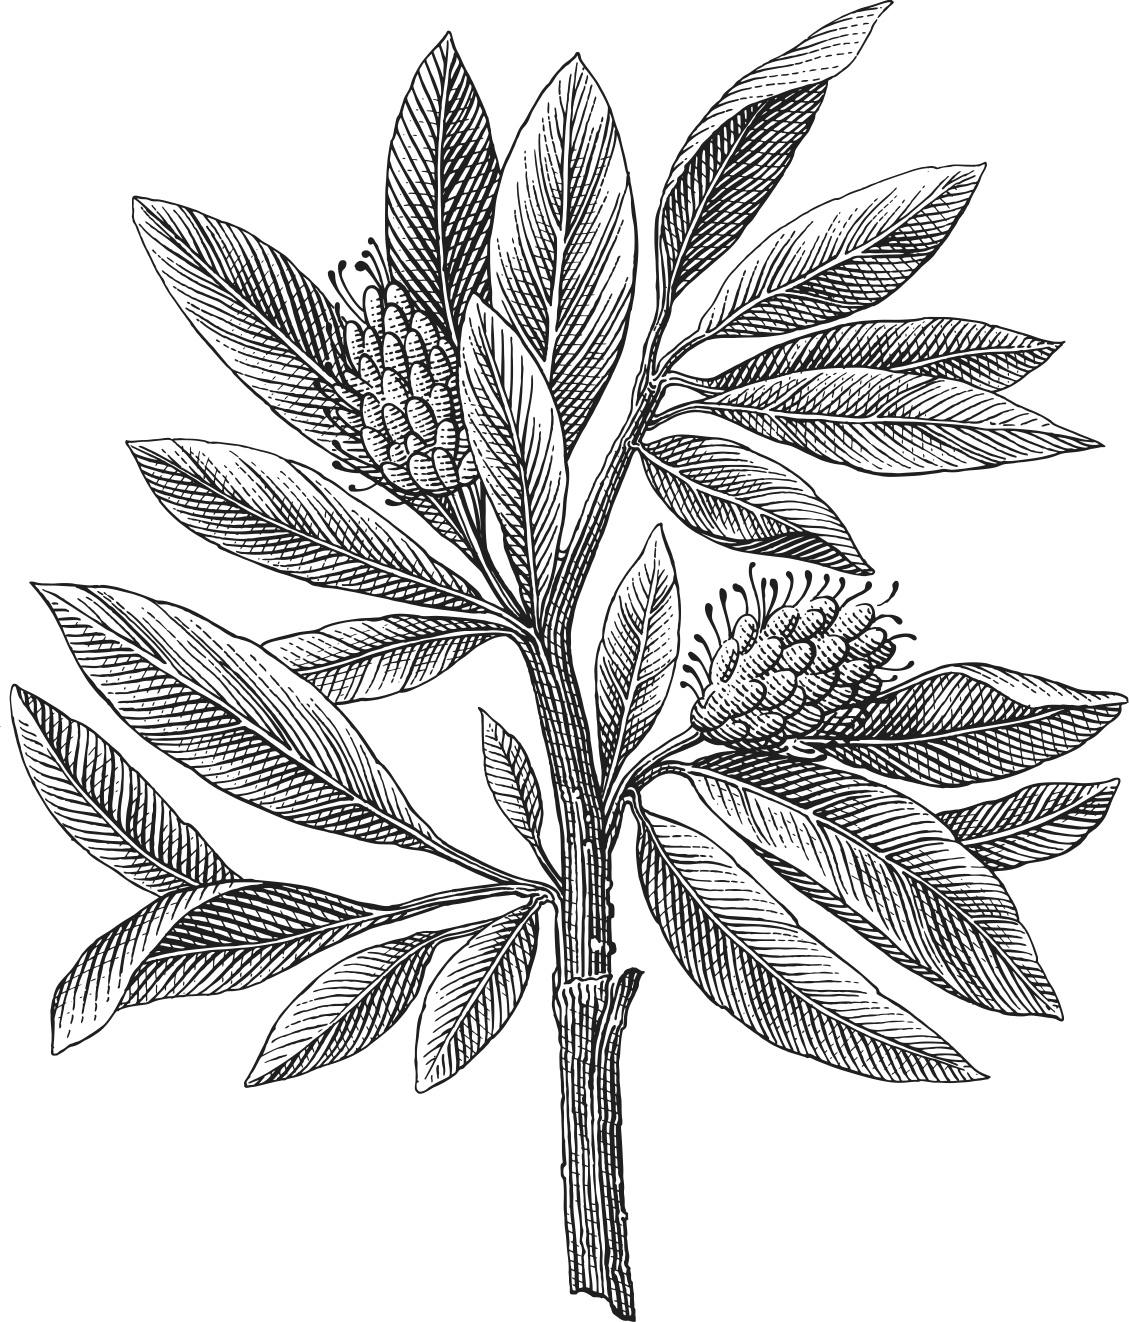
\includegraphics[keepaspectratio,scale=0.65]{lnu_etch.png} % Bakgrundsbild
    }
}
\newcommand\BackgroundPicLogo{
    \put(15,700){
    
\includegraphics[keepaspectratio,scale=0.10]{logo.png} % Logga i vänstra hörnet
    }
}

\newcommand{\horrule}[1]{\rule{\linewidth}{#1}} % Skapa hortisontell linje

\title{	\vspace{-10cm}
    \normalfont \normalsize
    \textsc{Linnaeus University} \\ [25pt] % Universitetes namn
    \horrule{0.5pt} \\[0.4cm] % Tunn linje högst upp
    \huge Seminar 4\\ % Arbetes titel
	\large \textcolor{gray}{1DV020 -- Server Administration}
    \horrule{0.5pt} \\[0.4cm] % Tunn linje längst ner
}

\author{Jacob Lindehoff} % Författarnas namn

\date{\normalsize\today} % Dagens datum

\begin{document}
\AddToShipoutPicture*{\BackgroundPic} % Lägger in backgrundsbild på första sidan
\AddToShipoutPicture*{\BackgroundPicLogo}
\maketitle % Skriv ut titeln
\noindent % Tabba inte in på första meningen

%------------------------------------------------
%	Introduktion
%------------------------------------------------
\section{Introduction}
  During this seminar, we will address the following topics:
\begin{itemize}
	\item Directory Services
	\item Active Directory
	\begin{itemize}
    	\item Overview
		\item DNS
		\item Global Catalog
		\item Organizational Units
		\item User accounts
		\item Groups
		\item User Profile
		\item Delegation of Administration
	\end{itemize}
    \item Access Control
    \item Group Policy
\end{itemize}

%------------------------------------------------
%	Deadline
%------------------------------------------------
\section{Deadline}
  The seminar is on the {\color{red}4th of March 2015} and it is compulsory. If you cannot participate, it must be notified in advance and a written report of the seminar must be submitted no later than {\color{red}3 days} after the seminar. The written report should contain detailed answers to all questions in the seminar.
  \newpage
%------------------------------------------------
%	Seminariefrågor
%------------------------------------------------
\section{Seminar Questions}

\subsection{Active Directory}
\begin{enumerate}
\begin{large}
	\item What is a directory service and what uses does it have?
	\item Describe the different parts of the Active Directory database.
	\item What is the Active Directory Schema and how many schema can be in an AD forest?
	\item What parts consist the logical and physical structure of and what you use them for?
	\item What is a domain controller?
	\item What is the Global Catalog and it's purpose?
	\item Why is a working DNS server so important for Active Directory?
	\item To create redundancy in a AD environment you install an additional domain controller. It is not enough, what you need to do more to allow users to log in if the first domain controller goes down?
	\item What is Organizational units and what is important to consider when creating their OU structure?
	\item What is implicit groups and how do you create one?
	\item Active Directory supports three group types, what are these?
	\begin{enumerate}[a.]
		\item Where can be members of those groups to come?
		\item Where can the different groups be used to give permissions?
	\end{enumerate}
	\item What is LDAP?
	\item What are the reasons you want to run with several different domain in a forest, it is not enough a domain?
	\item What distinguishes an Active Directory domain from a DNS domain?
	\item In what two ways can you run logon scripts in an AD environment and describe how to configure these?
	\item What does a user profile contain?
	\item How does "The roaming profile" work?
	\item Using OU you can delegate administration.
	\begin{enumerate}[a.]
		\item What are the different permissions can be put on an OU?
		\item How can this make it easier for an IT department?
	\end{enumerate}
	\setcounter{tmpc}{\theenumi}
	\end{large}
\end{enumerate}

\subsection{Access Control}
\begin{enumerate}
	\setcounter{enumi}{\thetmpc}
	\begin{large}
	\item What is A G DL P strategy, describe in detail and preferably with some examples?
	\setcounter{tmpc}{\theenumi}
	\end{large}
\end{enumerate}

\subsection{Group Policy}
\begin{enumerate}
	\begin{large}
	\setcounter{enumi}{\thetmpc}
	\item What is Group Policy?
	\item What can you apply GPO on?
	\item Which AD objects is affected by Group Policy?
	\item Can you apply a GPO in several different places?
	\item When are "Group Policy" settings applied?
	\item What happens if there is aconflicts between the group policy settings?
	\item What is meant by blocking the GPO inheritance on an OU?
	\begin{enumerate}[a.]
		\item How does it affect if you have set Enforced in a GPO?
	\end{enumerate}
	\item What is Group Policy Security Filtering?
	\begin{enumerate}[a.]
		\item Why should you avoid this?
	\end{enumerate}
	\item What is the following tools to?
	\begin{enumerate}[a.]
		\item gpupdate
		\item gpresult
	\end{enumerate}
	\item Select 10 different Group Policy settings that you find interesting and describe them.
	\end{large}
\end{enumerate}
\end{document}
